\begin{figure}
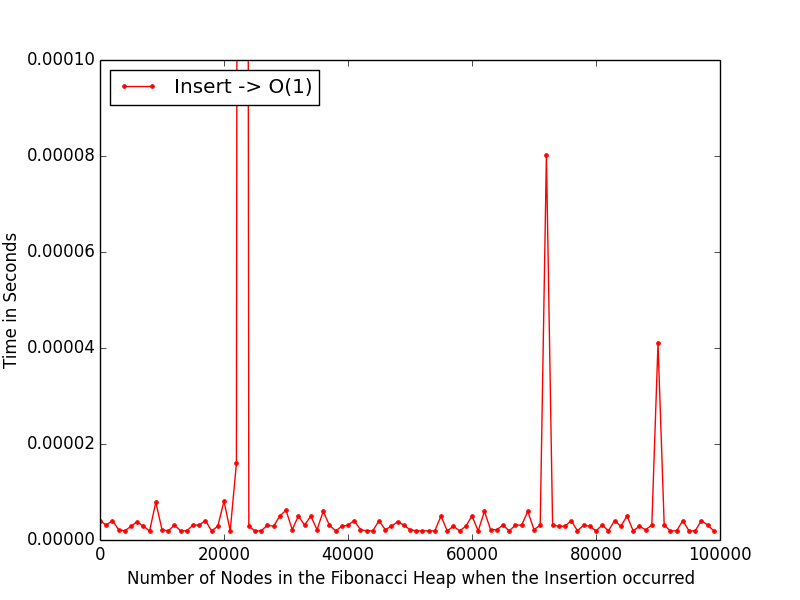
\includegraphics[width=0.95\columnwidth]{Figures/fibonacciHeapPerformanceInsert}
\caption{Insert Operation: $O(1)$}
\label{performanceInsert}
For Insertion operation, I created a new Fibonacci Heap with $n-1$ nodes and inserted the $n'^{th}$ node. Since it is constant time operation, we can observe that irrespective of the number of nodes added, the time taken to add the $n'^{th}$ node takes a constant time.
\end{figure}
\begin{figure}
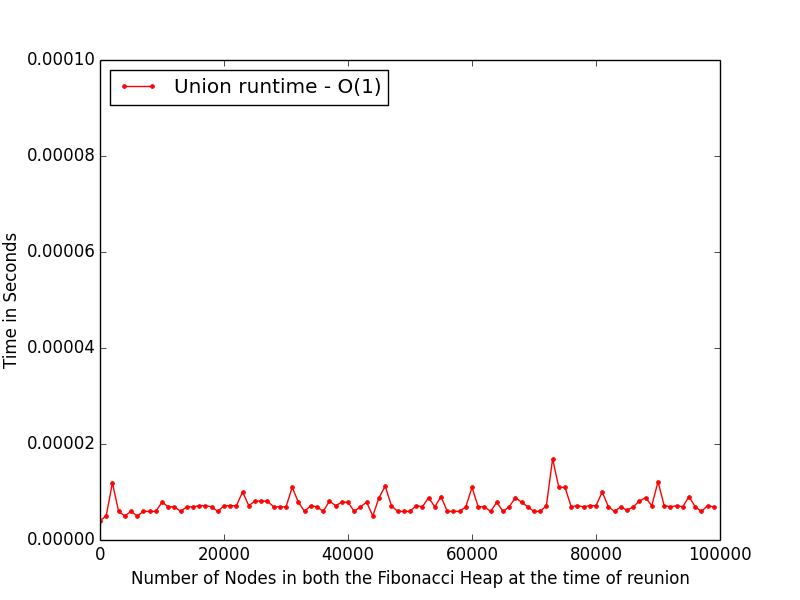
\includegraphics[width=0.95\columnwidth]{Figures/fibonacciHeapPerformanceUnion}
\caption{Union Operation: $O(1)$}
\label{performanceUnion}
For the Union operation, I created two Fibonacci Heap with $n$ nodes and then merged them. Since it is a constant time operation, we can observe that irrespective of the number of the nodes in both the Fibonacci Heap at the time of merging, the operation completes in a constant time.
\end{figure}
\begin{figure}
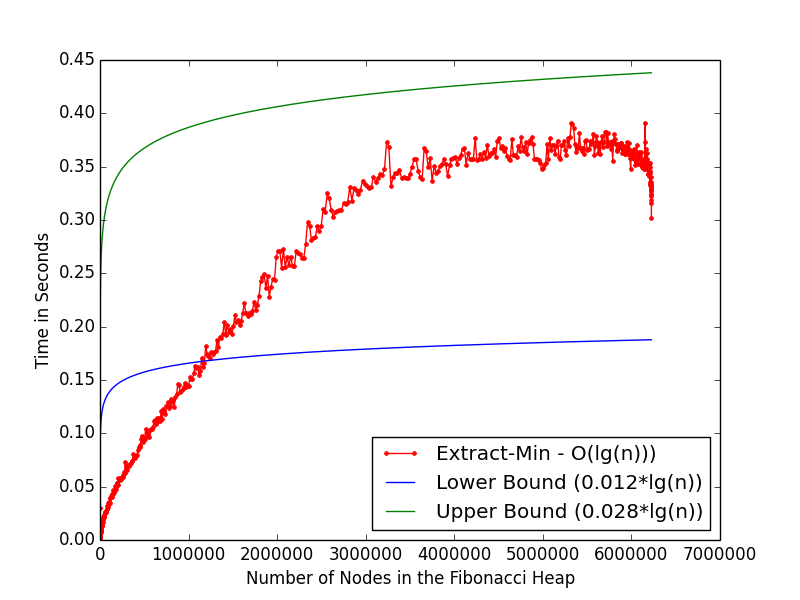
\includegraphics[width=0.95\columnwidth]{Figures/fibonacciHeapPerformanceExtractMin}
\caption{Extract Min Operation: $O(\log{n})*$}
\label{performanceExtractMin}
For the Extract-Min operation, I create just one Fibonacci-Heap and keep adding nodes to it and perform Extract-Min operation at various stages. Since it has an amortized time bound , the extract-min operation at any stage is dependent on the previous stage when the extract-min operation occurred and hence I decided to use just one Fibonacci Heap for the entire analysis. I have a lower and upper bound with a constant time $\log{n}$ which shows that Extract-Min has an amortized time bound of $O(\log{n})$
\end{figure}
\begin{figure}
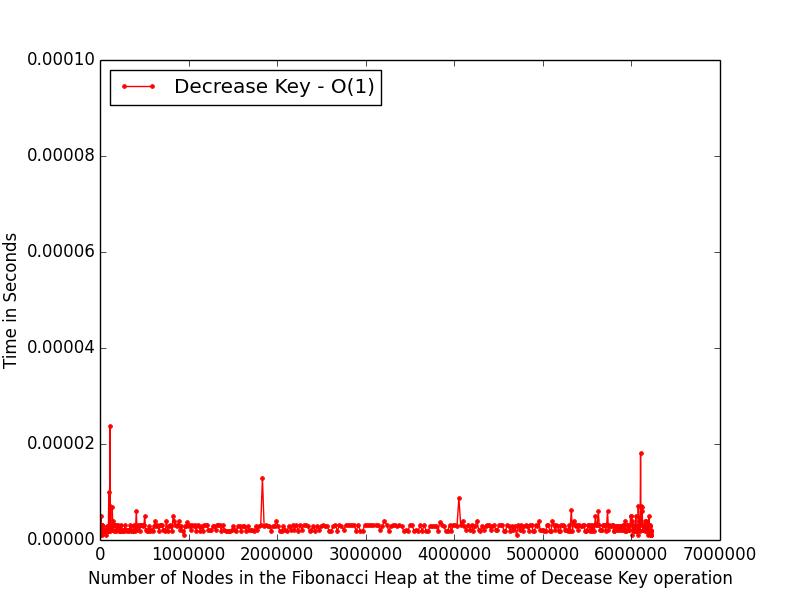
\includegraphics[width=0.95\columnwidth]{Figures/fibonacciHeapPerformanceDecreaseKey}
\caption{Decrease Key Operation: $O(1)*$}
\label{performanceDecreaseKey}
For the Decrease-Key operation, I create a Fibonacci-Heap and add nodes to it. At various stages, I perform the decrease-key operation. I use a single Fibonacci-Heap since decrease-key runtime bound is amortized. The current decrease key operation runtime is based on when the previous decrease key operation was performed.
\end{figure}
\begin{figure}
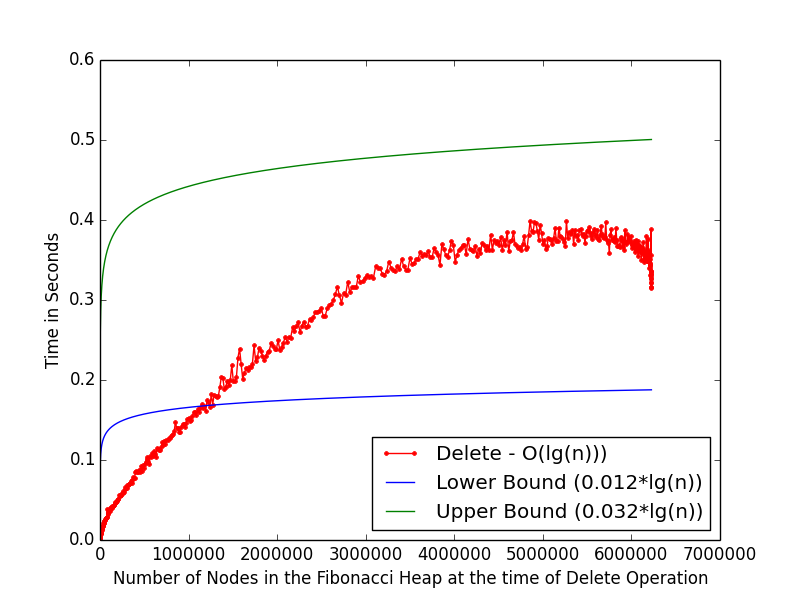
\includegraphics[width=0.95\columnwidth]{Figures/fibonacciHeapPerformanceDelete}
\caption{Delete Operation: $O(\log{n})*$}
\label{performanceDelete}
For the Delete operation, I create just one Fibonacci-Heap and keep adding nodes to it and perform delete operation at various stages. Since it has an amortized time bound, the delete operation at any stage is dependent on the previous stage when the delete operation occurred and hence I decided to use just one Fibonacci Heap for the entire analysis. I have a lower and upper bound with a constant time $\log{n}$ which shows that Delete operation has an amortized time bound of $O(\log{n})$
\end{figure}

